\documentclass[8pt,a4paper,compress]{beamer}
%\documentclass[8pt,a4paper,compress,handout]{beamer}

\usepackage{amsmath, amssymb, amsthm}
\usepackage{enumerate}
\usepackage{listings}
\usepackage{tikz}
\usetikzlibrary{shapes.gates.logic.US,trees,positioning,arrows,shapes.multipart}
\usepackage{wrapfig}

\usecolortheme{dove}
\useinnertheme{circles}
\beamertemplatenavigationsymbolsempty
\setbeamertemplate{headline}
{
  \leavevmode%
  \hbox{%
  \begin{beamercolorbox}[wd=\paperwidth,ht=6ex]{secsubsec}%
    \raggedright
    \hspace*{1.5em}%
    \normalsize
    \ifx\insertsection\empty\else
      \textbf{\insertsection\text{ }}%
      \ifx\insertsubsection\empty\else
        \textbf{$\bullet$\text{ }\insertsubsection}%
      \fi
    \fi
    \hspace*{2em}%
  \end{beamercolorbox}%
  }%
}
\setbeamerfont{frametitle}{size=\normalsize}
\setbeamertemplate{mini frames}{}
\setbeamertemplate{footline}[page number]

\definecolor{lightgray}{RGB}{240,240,240}
\definecolor{darkgreen}{RGB}{51,102,0}

\title{1.1 Your First Program}
\date{}

\lstset{
  backgroundcolor=\color{lightgray},
  basicstyle=\footnotesize\ttfamily,
  showstringspaces=false,
  commentstyle=\color{darkgreen},
  keywordstyle=\color{blue},
  stringstyle=\color{orange},
}

\begin{document}
\begin{frame}
\vfill
\titlepage
\end{frame}

\begin{frame}
\frametitle{Outline}
\tableofcontents
\end{frame}

\section{Programming in Java}
\begin{frame}[fragile]

\pause

\textbf{Our Programming Environment}
\begin{itemize}
\item Java Development Kit 7;  
\item BlueJ, a simple integrated development environment (IDE);
\item Terminal (aka console); and
\item Input and output libraries from the authors of our text. 
\end{itemize}

\pause
\smallskip

\textbf{Creating a Program} Use an editor or an IDE (eg, BlueJ) to create a file with \lstinline$.java$ extension containing the instructions for a Java program. 

\pause
\smallskip

\textbf{Compiling a Program} Translate a program from the Java language to a language (bytecode) more suitable for execution on the computer.

\begin{lstlisting}[language=bash]
$ javac P.java
\end{lstlisting}

\pause
\smallskip

\textbf{Running a Program} Use Java Virtual Machine (JVM) to direct the computer to follow the instructions in the bytecode.

\begin{lstlisting}[language=bash]
$ java P
\end{lstlisting}

\pause
\smallskip

\begin{center}
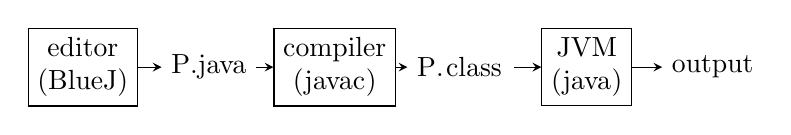
\begin{tikzpicture}
\begin{scope}[->,xshift=-7.5cm,yshift=-5cm,thin,
	   node distance=1.6cm,on grid,>=stealth,
  	   block1/.style={rectangle,draw,align=center},
	   block2/.style={rectangle,align=center}]
\node [block1] (1) {editor \\ (BlueJ)};
\node [block2] (2) [right=of 1] {\lstinline$P.java$};
\node [block1] (3) [right=of 2] {compiler \\ (\lstinline$javac$)};
\node [block2] (4) [right=of 3] {\lstinline$P.class$};
\node [block1] (5) [right=of 4] {JVM \\ (\lstinline$java$)};
\node [block2] (6) [right=of 5] {output};
\path (1) edge node [above] {} (2);
\path (2) edge node [above] {} (3);
\path (3) edge node [above] {} (4);
\path (4) edge node [above] {} (5);
\path (5) edge node [above] {} (6);
\end{scope}
\end{tikzpicture}
\end{center}
\end{frame}

\begin{frame}[fragile]
\pause

\textbf{Program 1.1.1} Hello, World

\begin{lstlisting}[language=Java]
public class HelloWorld {
    public static void main(String[] args) {
        System.out.println("Hello, World");
    }
}
\end{lstlisting}

\pause
\begin{lstlisting}[language=bash]
$ javac HelloWorld.java
\end{lstlisting}

\pause

\begin{lstlisting}[language=bash]
$ java HelloWorld
Hello, World
\end{lstlisting}

\pause
\smallskip

\textbf{Anatomy of a Program}
\begin{itemize}
\item Class definition; eg, \lstinline$public class HelloWorld {...}$.
\item Method definitions; eg, \lstinline$public static void main(String[] args)  {...}$.
\item Statements; eg, \lstinline$System.out.println("Hello, World")$.
\item Expressions; eg, \lstinline$"Hello, World"$.
\item Comments (multi-line \lstinline$/* ... */$ or single-line \lstinline$// ...$).
\end{itemize}

\pause
\smallskip

\textbf{Errors}
\begin{itemize}
\item Compile-time (syntax and semantic) errors.
\item Run-time errors (aka bugs).
\end{itemize}
\end{frame}

\section{Input and Output}
\begin{frame}[fragile]
\pause

\textbf{Command-line Arguments} List them after the program name when you run the program.

\begin{lstlisting}[language=bash]
$ java P arg_1 arg_2 ... arg_n
\end{lstlisting}

The arguments can be accessed within the \lstinline$main()$ method of  \lstinline$P$ via the array \lstinline$args$  as \lstinline$args[0]$, \lstinline$args[1]$, $\dots$, \lstinline$args[n - 1]$.

\pause
\smallskip

\textbf{Program 1.1.2} Using a command-line argument

\begin{lstlisting}[language=Java]
public class UseArgument {
    public static void main(String[] args) {
        System.out.print("Hi, ");
        System.out.print(args[0]);
        System.out.println(". How are you?");
    }
}
\end{lstlisting}

\pause

\begin{lstlisting}[language=bash]
$ java UseArgument Alice
Hi, Alice. How are you?
$ java UseArgument Bob
Hi, Bob. How are you?
\end{lstlisting}

\pause
\smallskip

\textbf{Bird's-eye View of a Java Program}
\begin{center}
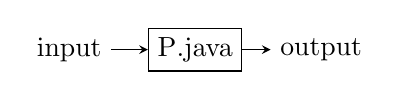
\begin{tikzpicture}
\begin{scope}[->,xshift=-7.5cm,yshift=-5cm,thin,
	   node distance=1.6cm,on grid,>=stealth,
  	   block1/.style={rectangle,draw,align=center},
	   block2/.style={rectangle,align=center}]
\node [block2] (1) {input};
\node [block1] (2) [right=of 1] {\lstinline$P.java$};
\node [block2] (3) [right=of 2] {output};
\path (1) edge node [above] {} (2);
\path (2) edge node [above] {} (3);
\end{scope}
\end{tikzpicture}
\end{center}
\begin{itemize}
\item Input types: command-line arguments, standard input, file input.
\item Output types: standard output, file output, graphical output, audio output.
\end{itemize}
\end{frame}

\end{document}
